\documentclass[12pt]{article}
\usepackage[utf8]{inputenc}
\usepackage{svg}
\usepackage{hyperref}
\usepackage{listings}
\usepackage{xcolor}
\usepackage{booktabs} % For prettier tables
\usepackage{multicol}
\usepackage{multirow}
\usepackage[shortlabels]{enumitem}
\usepackage{hyperref}
\usepackage{cleveref}
\usepackage{subcaption}
\usepackage{fancyhdr}
\usepackage{float}  
\usepackage{graphicx}
\usepackage{mhchem}
\graphicspath{ {./Figures/} }
\usepackage{array}
\usepackage{ragged2e}
\usepackage{multirow}
\usepackage{csquotes}
\usepackage{natbib}

\newcolumntype{P}[1]{>{\centering\arraybackslash}p{#1}} % center the column and justify its contents to the top in multirow tables
\newcolumntype{R}[1]{>{\RaggedLeft\arraybackslash}p{#1}} % Align column to the right in multirow tables

\definecolor{codegreen}{rgb}{0,0.6,0}
\definecolor{codegray}{rgb}{0.5,0.5,0.5}
\definecolor{codepurple}{rgb}{0.58,0,0.82}
\definecolor{backcolour}{rgb}{0.95,0.95,0.92}

\lstdefinestyle{mystyle}{
    backgroundcolor=\color{backcolour},   
    commentstyle=\color{codegreen},
    keywordstyle=\color{magenta},
    numberstyle=\tiny\color{codegray},
    stringstyle=\color{codepurple},
    basicstyle=\ttfamily\footnotesize,
    breakatwhitespace=false,         
    breaklines=true,                 
    captionpos=b,                    
    keepspaces=true,                 
    numbers=left,                    
    numbersep=5pt,                  
    showspaces=false,                
    showstringspaces=false,
    showtabs=false,                  
    tabsize=2
}

\lstset{style=mystyle}

% --- set footer and header ---
\renewcommand{\headrulewidth}{1pt}
\renewcommand{\footrulewidth}{1pt}
\pagestyle{fancy}
\fancyhf{}

\makeatletter\let\Title\@title\makeatother

\lhead{\Title}
\rfoot{
\includegraphics[height=1cm]{images/logo_small.png}} % right header logo
\setlength\headheight{16pt}
\setlength{\footskip}{50pt}
\lhead{\Title} %rightH title
\cfoot{\thepage}
% --- end footer and header ---

%----------EDIT COVER INFO HERE -----------------%

\def \LOGOPATH {images/ITU.svg}
\def \DEPARTEMENT {IT University of Copenhagen}
\def \COURSENUM {BSDSESM1KU}
\def \COURSENAME {DevOps, Software Evolution and Software Maintenance}
\def \REPORTTITLE {ITU-MiniTwit}
\def \STUDENTNAME {
    \begin{tabular}{@{}l@{\hspace{2em}}l}
        \textbf{Prepared by:} & Anton Vadsholt \texttt{<avad@itu.dk>}
        \\ & Atila Arianpour Wolff \texttt{<atia@itu.dk>}
        \\ & Karl Gustav Løhr \texttt{<kagl@itu.dk>} 
        \\ & Sebastian Graakjær Blok \texttt{<segb@itu.dk>}
        \\ & Silas Willendrup Wolff \texttt{<siwo@itu.dk>}
    \end{tabular}
    \vspace{0.5cm}
}




% Make subsubsubsection
\makeatletter
\newcommand{\subsubsubsection}[1]{\paragraph{#1}\mbox{}\\}
\makeatother

% \documentclass{article}

\usepackage{fancyhdr}
\usepackage{lastpage} % <--- ADD THIS!

\pagestyle{fancy}
\fancyfoot[C]{Page \thepage\ of \pageref{LastPage}}

\begin{document}

% Title Page
\begin{titlepage}
    \vfill
    \begin{center}
        \includesvg[width=0.7\textwidth]{\LOGOPATH} \\
        \hfill \\
        \Large{\DEPARTEMENT} \\
        \Large{\COURSENUM\;-\;\COURSENAME} \\
        \vfill
        \textbf{\LARGE{\REPORTTITLE}}
    \end{center}
    \vfill
    \begin{flushleft}
        \Large{\STUDENTNAME} \\
        \Large{\INSTRUCTOR} \\
    \end{flushleft}
    \vfill
    \begin{center}
        \Large{\textbf{Date:} \today}
    \end{center}
\end{titlepage}

%\newpage
%\input{Sections/Abstract}

\newpage
\tableofcontents

\newpage
%A description and illustration of the:

%Design and architecture of your ITU-MiniTwit systems

%All dependencies of your ITU-MiniTwit systems on all levels of abstraction and development stages. That is, list and briefly describe all technologies and tools you applied and depend on.

%Important interactions of subsystems.
    %For example, via an illustrative UML Sequence diagram that shows the flow of information through your system from user request in the browser, over all subsystems, hitting the database, and a response that is returned to the user.
    
    %Similarly, another illustrative sequence diagram that shows how requests from the simulator traverse your system.

%Describe the current state of your systems, for example using results of static analysis and quality assessments.

\section {System's Perspective}
\subsection{Design and Architecture}

\begin{figure}[H]
    \centering
    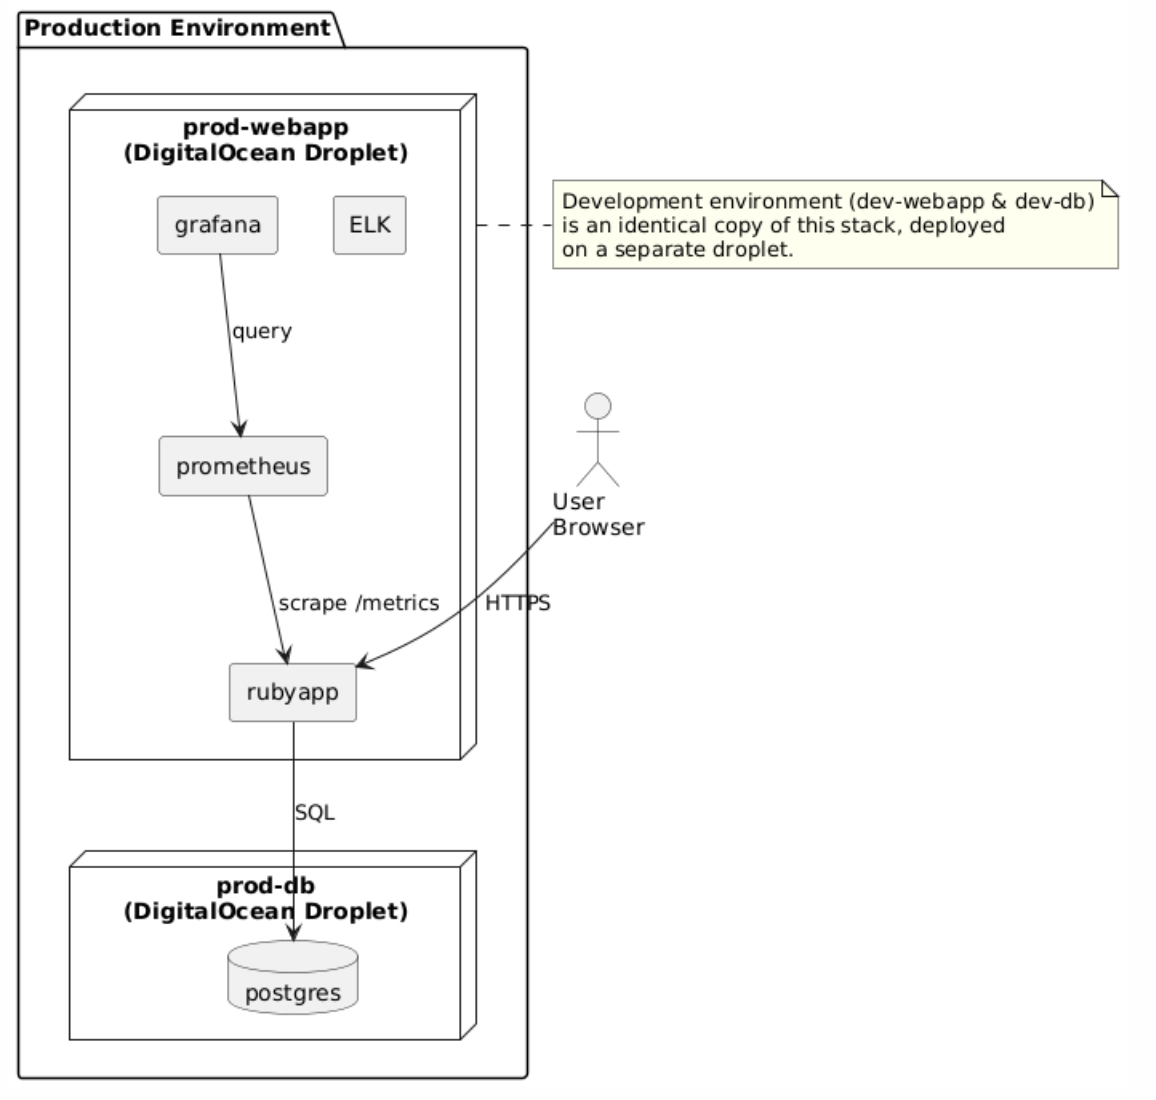
\includegraphics[width=1\linewidth]{images/deployment_diagram.png}
    \caption{Deployment Diagram}
    \label{fig:deployment}
\end{figure}

Figure~\ref{fig:deployment} presents the deployed architecture of \textit{MiniTwit} in production. The application uses 2 DigitalOcean droplets: 1 for application logic and 1 for a database. Splitting the droplets follows the principle of separation of concerns, as the webapp droplet is responsible for all logical tasks, as well as logging and monitoring, and the db droplet is only responsible for storage. Additionally this keeps our data safe, if the webapp droplet was harmed. \\

The application logic is build in Ruby and the database uses PostgreSQL as a database management system. We use ELK stack for logging, and Grafana with Prometheus for monitoring. \\

All these systems are containerized using docker. For example, postgres is not directly installed on the db droplet. Instead, a container is running of a docker image with support for postgres. The same goes for the webapp, logging and monitoring. The monitoring is 2 systems, grafana and prometheus, each running in their own containers. Grafana is for visualizing the data, and prometheus is a database, that keeps time-series data, that can then be queried to give insight into the activity. \\


\subsection{Dependencies}

Here follows a full list of all dependencies our systems rely on, with a short description of its purpose:

\subsubsection{Core Application Dependencies}
\begin{itemize}
    \item \textbf{sinatra} -- Web framework (similar to Flask in Python)
    \item \textbf{sequel} -- Database toolkit and ORM
    \item \textbf{sqlite3} -- SQLite database adapter
    \item \textbf{bcrypt} -- Password hashing
    \item \textbf{rack} \& \textbf{rack-test} -- Web server interface and testing
    \item \textbf{puma} -- Web server
    \item \textbf{pg} -- PostgreSQL adapter
    \item \textbf{rackup} -- Rack server launcher
    \item \textbf{rspec} -- Testing framework
    \item \textbf{rest-client} -- HTTP client library
\end{itemize}

\subsubsection{Database}
\begin{itemize}
    \item \textbf{Sequel gem} - ORM
    \item \textbf{PostgreSQL}
    \begin{itemize}
        \item Main production database, running off of a docker image
    \end{itemize}
    \item \textbf{SQLite3}
    \begin{itemize}
        \item Local database for testing, uses SQLite 3 module gem
    \end{itemize}
\end{itemize}

\subsubsection{Development \& Testing Dependencies}
\begin{itemize}
    \item \textbf{Testing Frameworks}
    \begin{itemize}
        \item \textbf{rspec} -- Ruby testing framework
        \item \textbf{dawnscanner} -- Security scanner
        \item \textbf{fasterer} -- Ruby performance analyzer
        \item \textbf{rubocop} -- Consistent code standards, style guide and formatting
    \end{itemize}
\end{itemize}

\subsubsection{CI/CD}
\begin{itemize}
    \item \textbf{Github Actions} used as the CI/CD platform for all workflows, and use the following templates:
    \begin{itemize}
        \item \textbf{actions/checkout@v4} -- Code checkout
        \item \textbf{ruby/setup-ruby@v1} -- Ruby environment setup
        \item \textbf{appleboy/ssh-action@v0.1.10} -- SSH deployment
        \item \textbf{softprops/action-gh-release@v1} -- GitHub release management
    \end{itemize}
\end{itemize}

\subsubsection{Development Environment}
\begin{itemize}
    \item \textbf{Vagrant Configuration}
    \begin{itemize}
        \item Digital Ocean provider
        \item Ubuntu 22.04 base image for both webapp and db
        \item Docker and Docker Compose installation
    \end{itemize}
\end{itemize}

\subsubsection{Security Dependencies}
\begin{itemize}
    \item \textbf{bcrypt} -- Password hashing
    \item \textbf{dawnscanner} -- Security scanning
\end{itemize}

\subsubsection{Monitoring \& Health Checks}
\begin{itemize}
    \item PostgreSQL health checks in Docker
    \item Database connection monitoring
    \item GitHub Actions for automated testing and deployment
\end{itemize} 

\subsection{Interactions of Sub-systems}

\begin{figure}[H]
    \centering
    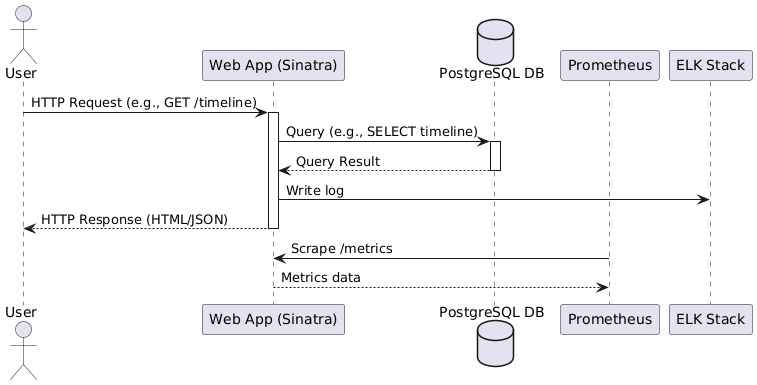
\includegraphics[width=1\linewidth]{images/sequence_user.png}
    \caption{sequence-user}
    \label{fig:seq-user}
\end{figure}

Figure~\ref{fig:seq-user} illustrates how a user-request flows through the deployed \textit{MiniTwit} system. When a user makes a request, for example accessing their timeline, the request is handled by the \texttt{webapp}, a Sinatra-based web application running as a container from a docker image. The application queries a PostgreSQL database for whatever data needed to fulfill the users request. \\

These request are directly relevant to serving the user's request, but also cause other effects. Sinatra sends data to out logging system and our monitoring system, to capture the activity it receives. The way it does logging, is similar to a print statement to standard output, but uses a specialized database, for handling these. For monitoring, we have an endpoint, '/metrics', dedicated to accumulating data, that Prometheus then captures and stores.\\

On top of this, we have api-endpoints, that allow automated systems to use the system without going through the UI. For example, the simulator will be using these endpoints. The flow of information after the requests, will be the same as for a user-request. 

\subsection{State of the system}

\begin{figure}[H]
    \centering
    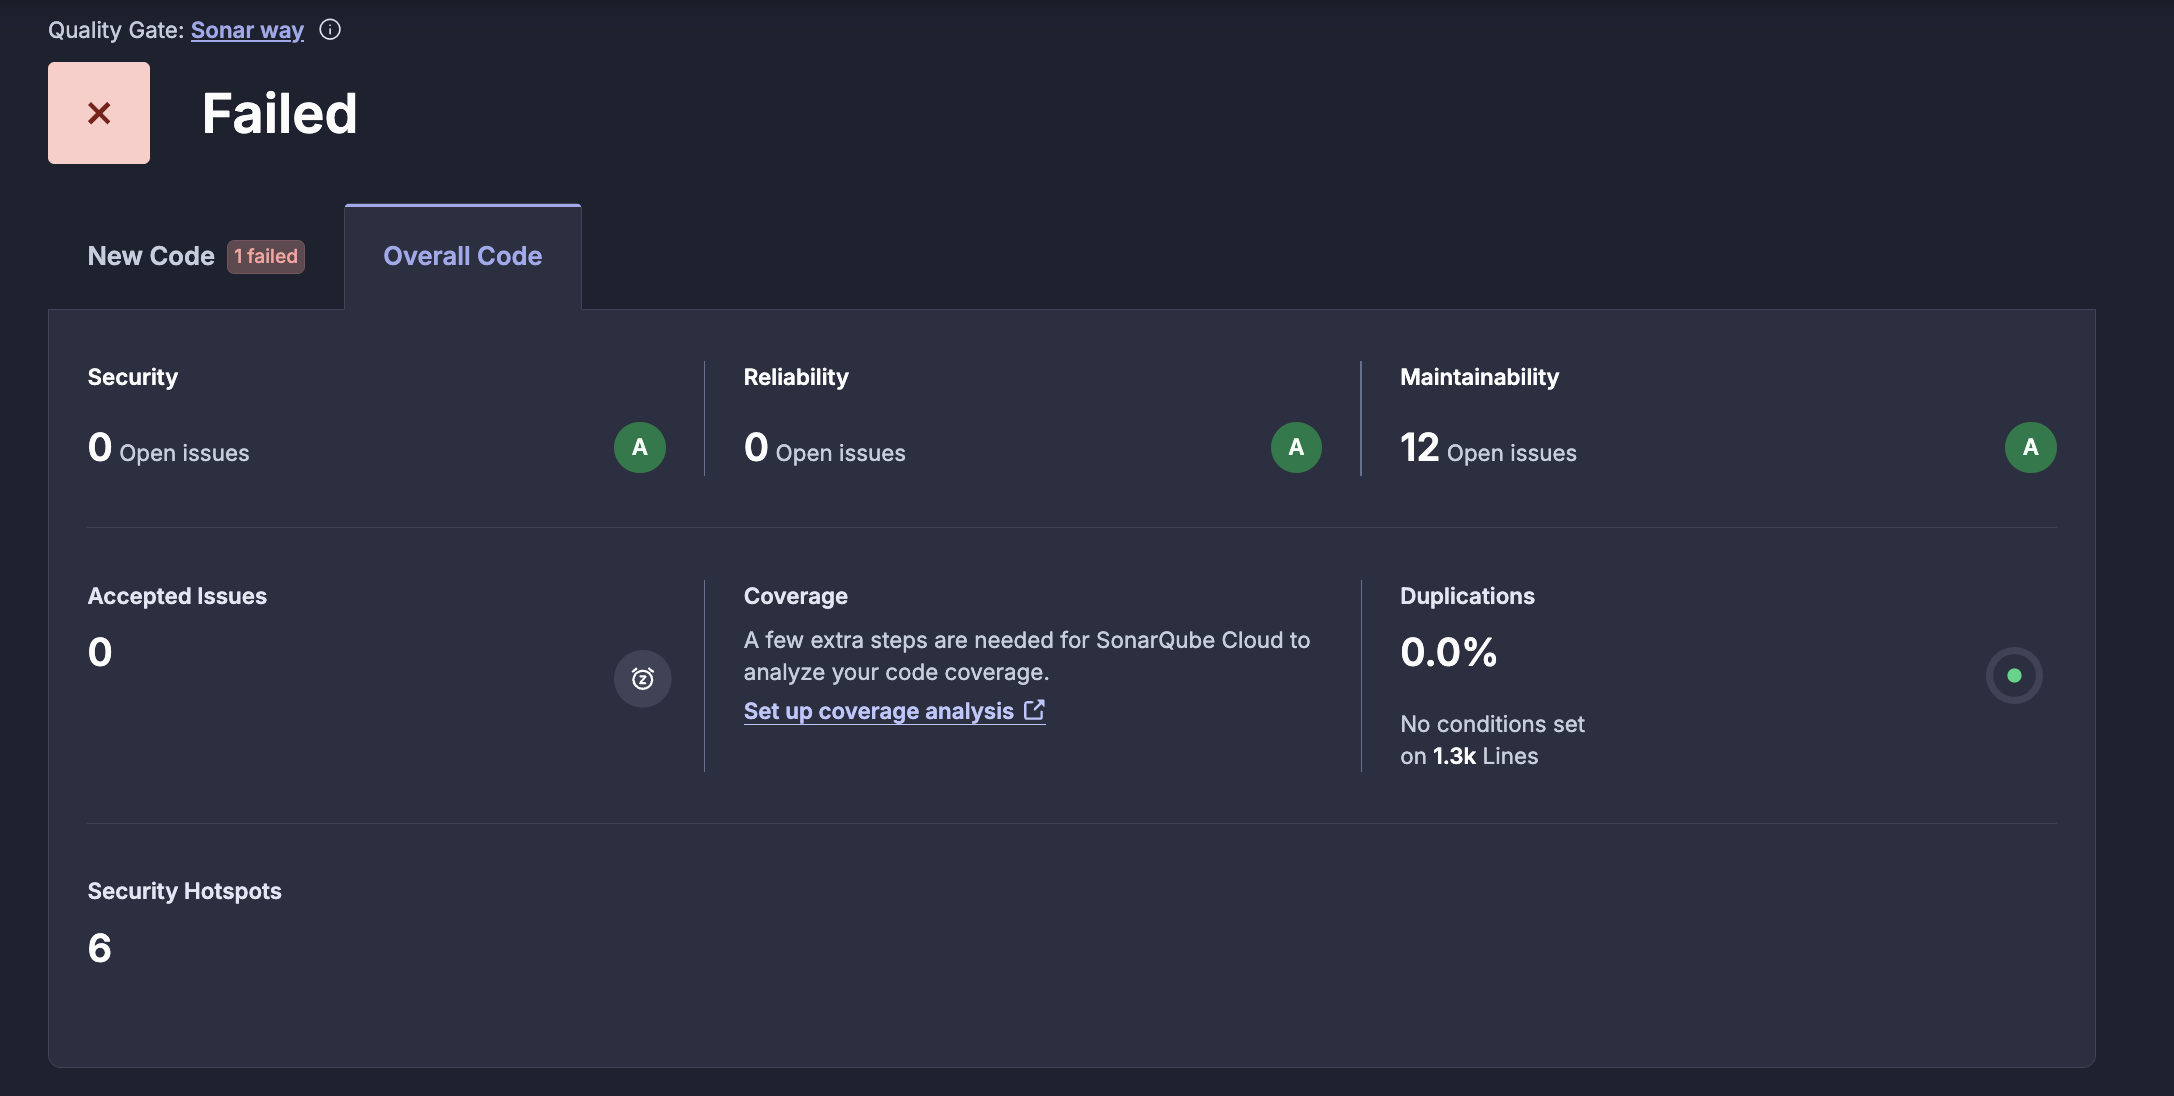
\includegraphics[width=1\linewidth]{images/sonarqube.png}
    \caption{SonarQube}
    \label{fig:sonarqube}
\end{figure}

We've used SonarQube for code analysis, in order to asses the quality of our code, for example in terms of maintainability, and to prevent human errors. As the figure \ref{fig:sonarqube} shows, we have a reasonably solid codebase, with some room for improvement. \\

First lets address the 6 Security Hotspot issues. 4 of these are related to the flag\_tool.cs file, which is not exposed to the internet anyway. The 2 others are about our docker containers running as root: \\

\begin{figure}[h]
  \centering
  \begin{minipage}[t]{0.45\linewidth}
    \centering
    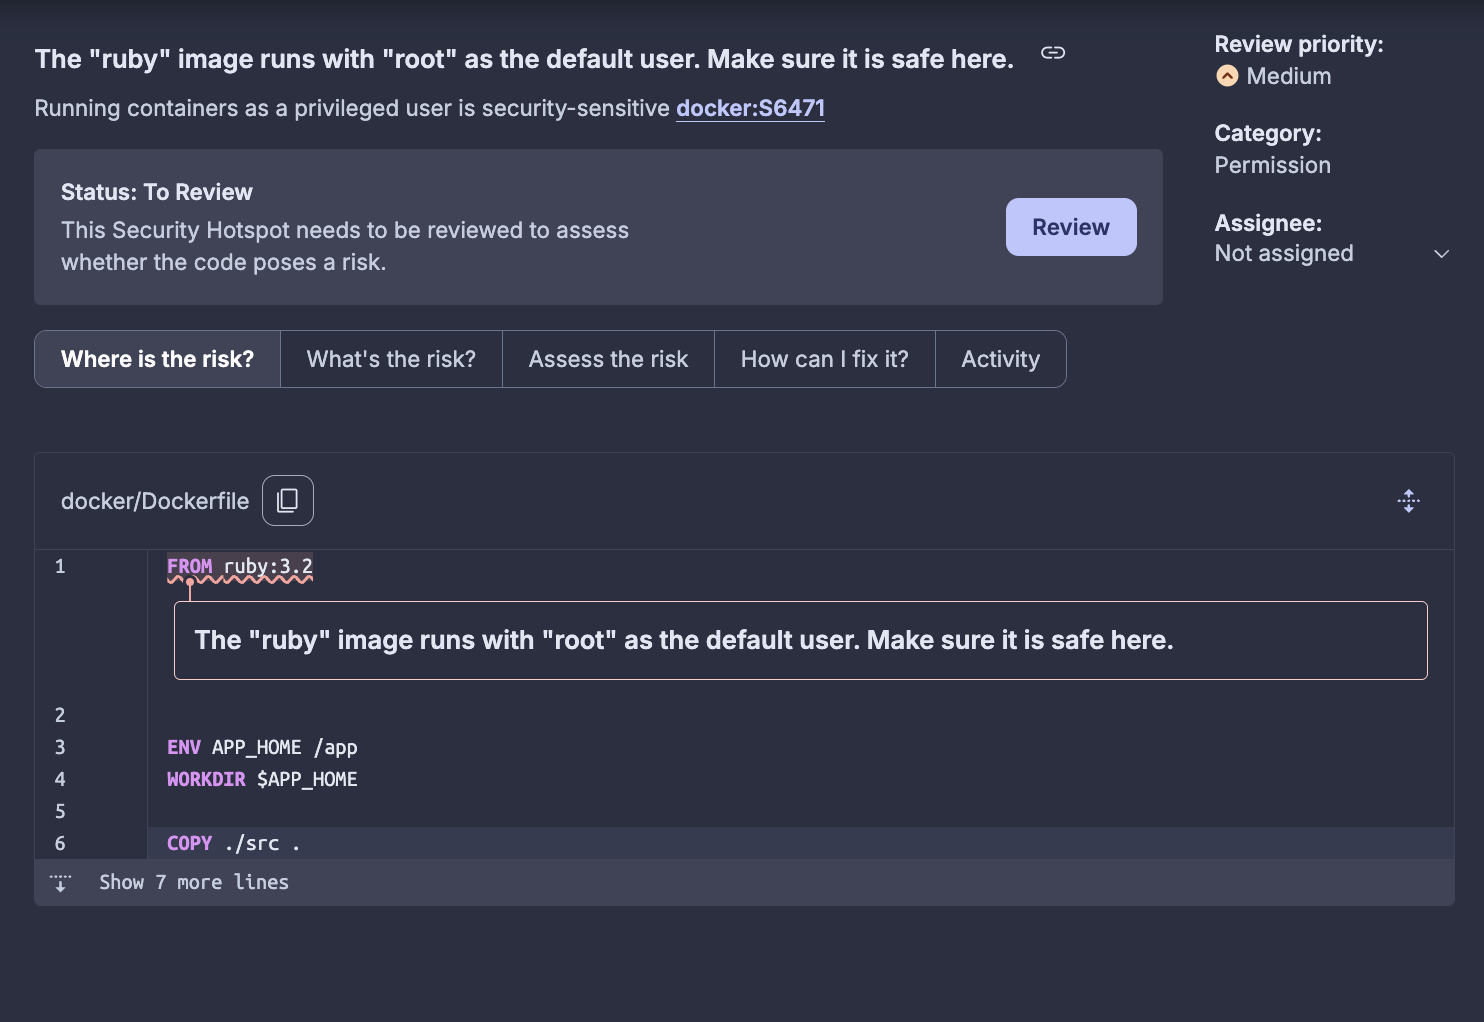
\includegraphics[width=0.9\linewidth]{images/sonarqube-ruby.png}
    \caption{Ruby container warning}
    \label{fig:ruby-warning}
  \end{minipage}%
  \hfill
  \begin{minipage}[t]{0.45\linewidth}
    \centering
    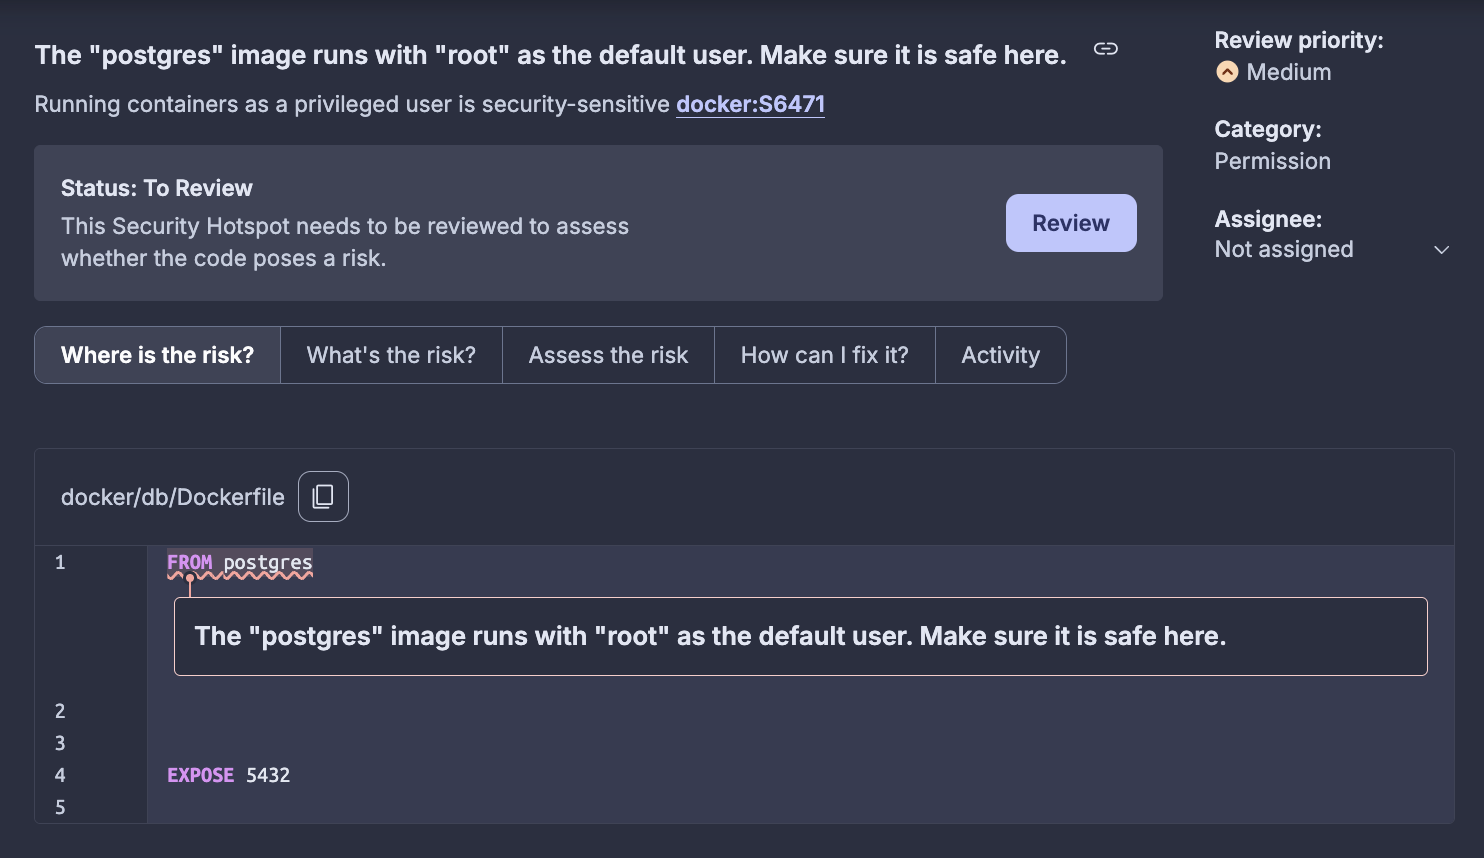
\includegraphics[width=0.9\linewidth]{images/warning_docker.png}
    \caption{PostgreSQL warning}
    \label{fig:postgres-warning}
  \end{minipage}
\end{figure}

Both warnings are about the default user being \texttt{root} inside the containers. We believe this to be a low-risk issue, because the containers run in isolated Docker environments without elevated host privileges or sensitive bind mounts. The web application interacts with the database exclusively through the Sequel ORM, and the PostgreSQL container is password-protected. While using a non-root user is a recommended hardening step, we determined that the current configuration does not introduce meaningful risk. \\

For maintainability issues, 8 of these are for flag\_tool.c, and 2 are for refactored\_minitwit\_tests.py, both files are not maintained, and thus not an issue. The last error is regarding a string literal used 3 times, which could be made into a variable. We believe this is manageable. \\


%This perspective should clarify how code or other artifacts come from idea into the running system and everything that happens on the way.

%In particular, the following descriptions should be included:

    %A complete description of stages and tools included in the CI/CD chains, including deployment and release of your systems.

    %How do you monitor your systems and what precisely do you monitor?

    %What do you log in your systems and how do you aggregate logs?

    %Brief results of the security assessment and brief description of how did you harden the security of your system based on the analysis.
    
    %Applied strategy for scaling and upgrades.
    
%In case you have used AI-assistants during your project briefly explain which system(s) you used during the project and reflect how it supported or hindered your process.



\section{Process' perspective}

\subsection{CI/CD Workflow}

\begin{figure}[H]
    \centering
    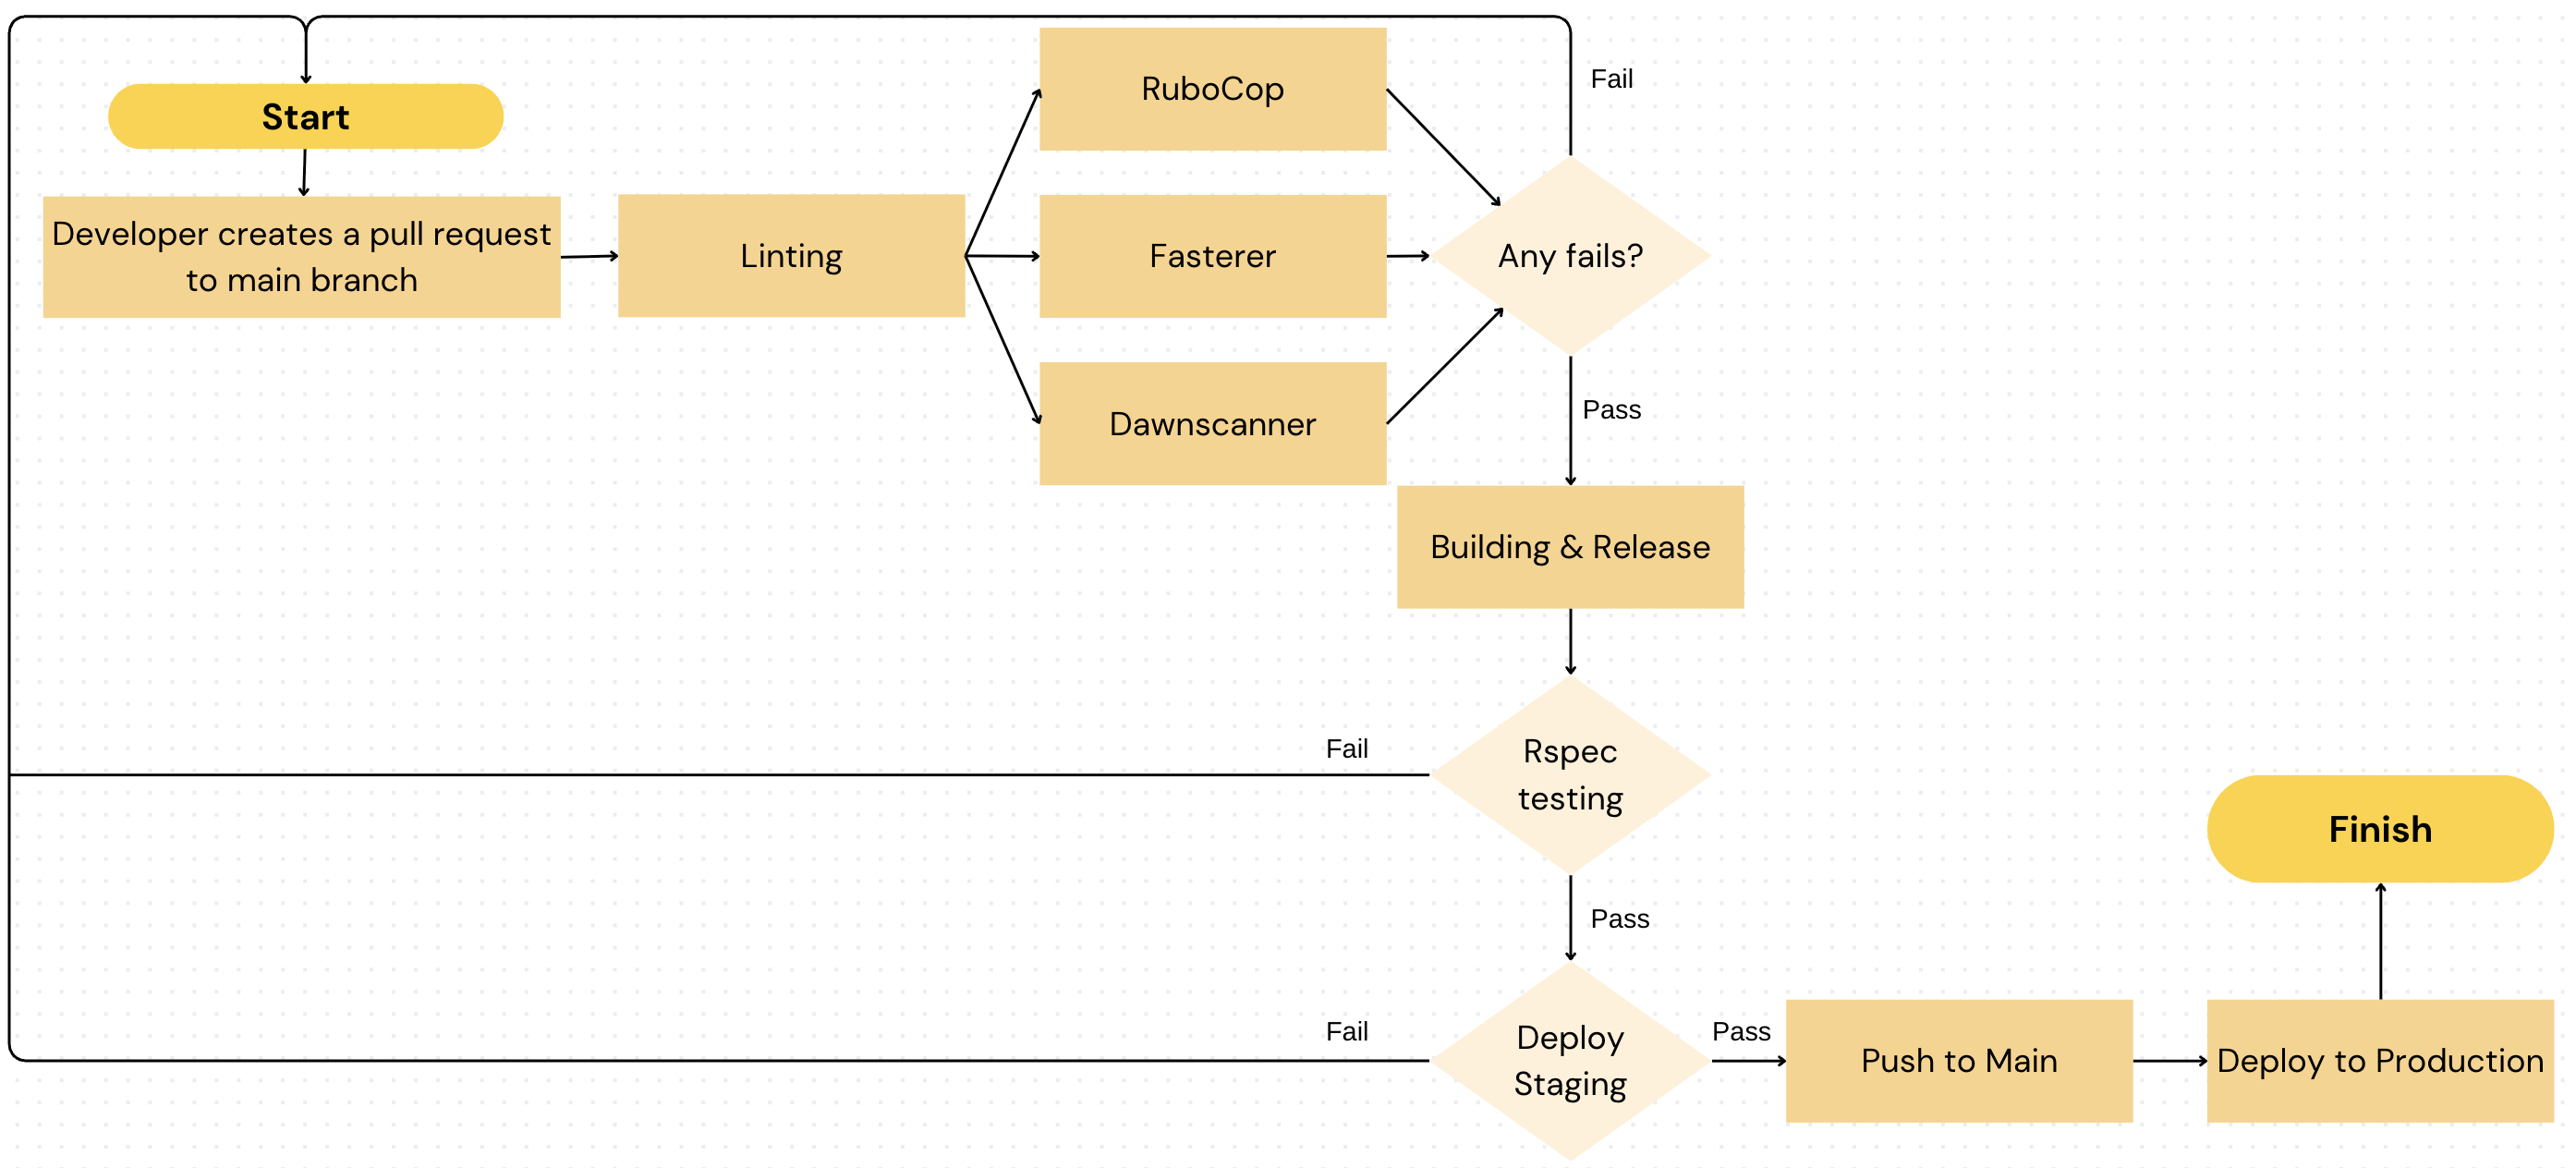
\includegraphics[width=1\linewidth]{images/Workflow.png}
    \caption{CI/CD workflow}
    \label{fig:Workflow}
\end{figure}
Figure~\ref{fig:Workflow} shows the overall CI/CD workflow. Our pipeline is implemented using GitHub Actions, which automates the process of linting, building, testing, and deploying the system upon each pull request to the \texttt{main} branch. 

\subsubsection{Continuous Integration: Test and Build}
Every pull request to \texttt{main} triggers the CI pipeline starting the linting tools. \texttt{RuboCop} Checks for style violations and enforces coding standards. It has the lowest risk but it also easier to fix as it suggests auto-fixes for most of the recommendations. \texttt{Fasterer} analyzes the code for inefficient patterns and suggests performance improvements. It is static and fast, but it’s focused on optimization, not correctness. It runs after style checks to catch possible refactors. \texttt{Dawnscanner} performs a static security audit, flagging potential vulnerabilities in our Ruby codebase. This is the most impactful check if vulnerabilities are found because security scans can be more computationally expensive and less frequent in early development, but critical before any merge or deploy. Finally, we also use SonarQube in our pipeline. This tool catches both security flaws and code smells, that could make our code less maintainable. \\

After passing all static analysis tools, our CI pipeline build the docker image an creates a release. The release is used for the unit and integration test. It runs \texttt{Rspec} to execute the test suite to ensure that our application logic is functioning as intended before moving on. If any \texttt{Rspec} test fails, the pipeline stops, and deployment is halted. This fail-fast strategy prevents broken code from reaching staging or production. 
The docker image build is later used for stage deployment(see section \ref{CD-sec}).

\subsubsection{Continuous Deployment}\label{CD-sec}

\begin{figure}[H]
    \centering
    
\includegraphics[width=1\linewidth]
    {images/CD.png}
    \caption{CD-Pipeline}
    \label{fig:CD}
\end{figure}

Figure~\ref{fig:CD} is the CD pipeline and illustrates how the staging works for the development environment and production. Our Continuous Deployment pipeline is defined as a GitHub Actions workflow triggered on pushes to the \texttt{main} branch. It performs automated end-to-end deployment using Docker and DigitalOcean Droplets. \\

After building Docker images for the web and database services using \texttt{docker compose}, the images are tagged and pushed to DockerHub. From there, the pipeline establishes SSH connections to two separate production servers: one for the PostgreSQL database, and one for the Ruby-based web application. \\

On the database server, the pipeline stops and removes existing containers, pulls the latest image, and redeploys the database using environment variables and persistent storage. \\

On the application server, the pipeline pulls the latest web image, runs Sequel database migrations, and then starts the application container with the required environment configuration. Finally, we use a curl-based HTTP check to verify the service is online. \\

This pipeline ensures fast, repeatable deployments and minimizes manual errors. We use secrets and environment variables to secure sensitive credentials and configuration data throughout the workflow.


\subsection{Monitoring}
To ensure the health, performance, and observability of our MiniTwit system, we implemented a multi-layered monitoring setup combining container health checks, application-level instrumentation, and Prometheus-based scraping.
For healthchecks we use Docker’s built-in healthcheck functionality to monitor the readiness of the PostgreSQL database. With a 5-second interval and 3-second timeout, retrying up to 5 times. This check ensures the database is reachable before the frontend service attempts to connect, which helps prevent runtime errors caused by timing issues during container startup. To make sure the application only starts once the database is healthy, the condition \texttt{service\_healthy} is used for improving stability in both development and deployment environments. \\

Our Ruby web application-level monitoring is implemented using the prometheus-client gem and a custom middleware \texttt{MetricsHelper} that captures \textbf{HTTP response counts}, labeled by status, HTTP method, and \textbf{request durations}, measured in milliseconds. These metrics are exposed via a /metrics endpoint in Prometheus text format, which Prometheus scrapes at regular intervals. \\

Our Prometheus is configured via prometheus.yml to scrape metrics from The webapp container and itself, \textbf{prometheus:9090} for internal health. We use 5-15 second scrape intervals for near real-time visibility.


\subsection{Logging}

We implemented logging using the ELFK stack. The stack helps us build and collect structured logs, that we can store and query, to get an overview of activity on the service. We have made a log-folder that lives in our docker containers, and is mounted in a droplet, to retain the data. The log-folder contains files like:

\begin{itemize}
    \item Debug
    \item Info
    \item Warning
    \item Error
    \item Fatal
    \item unknown
\end{itemize}

This structure helps us easily identify the best logs for finding and solving problems for debugging or optimization, or even just curiosity about what our users are doing on the site. We log things like status codes, http requests, and timestamps. Kibana creates visualizations across the log-files. \\


\subsection{Security}
When looking at our security, our main assets are the containers, that are exposed to the internet. This is both the webapp, the monitoring system, the logging system and the database. However, monitoring, logging and the database, only expose specific ports, and are password protected. This ensures that our data cannot be seen and modified by malicious actors.\\

The web application interacts with the database using an ORM layer, 'Sequel' in our case, which helps mitigate SQL injection by ensuring proper query parameterization. Similarly, the templating system used for rendering HTML, 'Embedded Ruby - .erb' in our case, escapes user input by default, which protects against common Cross-Site Scripting (XSS) attacks. \\

To keep sensitive environment variables, like access-tokens, passwords and private keys, secure, we use GitHub secrets. This way, we can store secrets, and use them in workflows, without exposing them to the world, in our repository. 


\subsection{Scaling and reliability}
To improve scalability and reliability for our application, we utilize Docker Swarm. Docker Swarm allows us to define a logic for managing Docker containers, like how they share/sync data between them, or if they simply have a central database and leader-node, as is the case for us.\\

In our setup, we maintain a central PostgreSQL database hosted on a dedicated, isolated Droplet, while the application containers are managed from another central Droplet. \\

Swarm provides automatic load balancing by distributing incoming requests across available replicated containers. It also offers fault tolerance by rescheduling affected services elsewhere in the cluster, if a container crashes or becomes unavailable. This orchestration simplifies scaling and improves the robustness of our deployment.

\section{Reflection Perspective}

The biggest change to our workflow from before we gained this experience with DevOps, also representing our style of DevOps, is how an extensive pipeline empowers a developer to take more control of his own work. Usually, our group-work required a lot of checking in with the other developers, to make sure we are on the same page about how solutions are implemented, and ensuring we each agree on, and live up to the same quality and style standards. With an extensive pipeline, a lot of this can be alleviated by specific steps, that give a much stronger guarantee, and a stronger sense of confidence, that the code i am personally working on, is going to be fitting for the project, and the other developers, without waiting for, or maybe even interrupting, the other developers for confirmations. \\

An example of this are things like linting tools and static code analysis. These are tools that we use to inspect our code for problems regarding its style and maintainability. By building them into the pipeline, a developer will be notified of ways his code might breach the established standards, so he can fix them before merging code. This greatly reduces the need for code-reviews, which is a very concrete example, of how a developer more easily can stand by his own work all the way through delivery, without wasting time and energy by having another developer sign off on it. \\

This benefit is not limited to upholding good coding standards, but is as helpful in terms of sharing competencies. An issue we've experienced in earlier projects, is how specific skills accumulate with the developers that have worked the most with a specific area, which can make it difficult for developers to switch what they work on. Say, i have written some code. Now i might not feel confident in pushing it to production, because another developer has been in charge of managing the production environment, including the vps/droplet or how we build or something similar. By building a workflow, that essentially captures all the knowledge required, to safely deliver my new work to the production environment, or whatever needs to be done with it, i can now deliver my work to production myself, without causing errors, or disturbing the developer, who initially setup the environment i want to use. This way, both of us are more productive. \\

These are examples of how a DevOps mindset, and DevOps tooling, has allowed each developer to take more independent ownership of their work, and streamline our co-operation. 


%\bibliographystyle{IEEEtran}
%\cleardoublepage
%\phantomsection
%\addcontentsline{toc}{section}{References}
%\bibliography{IEEEabrv,cites}


\end{document}
